\chapter{Ricerca euristica}

La ricerca esaustiva non è praticabile in problemi di complessità esponenziale (e.g.\ 10\textsuperscript{120} configurazioni in scacchi).\
Noi usiamo la conoscenza del problema e l'esperienza per riconoscere i cammini più promettenti:\ usiamo una stima del costo futuro \textit{evitando di generare gli altri} (pruning)!

La conoscenza euristica (dal greco ``eureka'') aiuta a fare scelte ``oculate'':\ non evita la ricerca, ma la riduce e in genere consente di trovare una \textbf{buona} soluzione in tempi accettabili.\
Sotto certe condizioni garantisce completezza e ottimalità.

\section{Funzioni di valutazione euristica}

Conoscenza del problema data tramite una \textit{funzione di valutazione f}, che include \textit{h} detta funzione di valutazione euristica:

\[h : n \rightarrow R\]

\noindent La funzione si applica al nodo ma dipende solo dallo stato (\textit{n}.Stato).\
\textit{g} dipendeva anche dal cammino fino al \textit{nodo}.

\[f(n) = g(n) + h(n)\]
dove $g(n)$ è il costo cammino visto con UC.

\subsubsection{Esempi di euristica \textit{h}}

Per procedere preferibilmente verso il percorso migliore, seguendo ``problem-specific information'', di stima del costo futuro:\ la città più vicina (o la città più vicina alla mèta in linea d'aria) nel problema dell'itinerario, il numero delle caselle fuori posto nel gioco dell'otto, il vantaggio in pezzi nella dama o negli scacchi.

\begin{figure}[H]
	\centering
	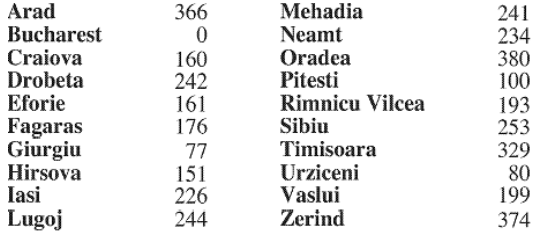
\includegraphics[width=0.5\textwidth]{immagini/Romania_euristica.png}
	\caption*{Mappa Romania:\ distanza in linea d'aria}
\end{figure}

\subsection{Algoritmo di ricerca Best-First}

\textbf{Best first} - heuristic \textit{con stesso algoritmo di UC} ma con uso di \textit{f} (stima di costo) per la \textit{coda con priorità}.\
La scelta di \textit{f} determina la strategia di ricerca:\ a ogni passo si sceglie il nodo sulla frontiera per cui il valore della \textit{f} è migliore (\textit{il nodo più promettente}).\

\noindent\textbf{Nota}:\ migliore significa ``minore'' in caso di un'euristica che stima la distanza della soluzione.\
Caso speciale:\ \textbf{greedy best-first}, si usa solo \textit{h} ($f=h$).

\subsubsection{Ricerca greedy best-first:\ esempio $f=h$}
\begin{figure}[H]
	\centering
	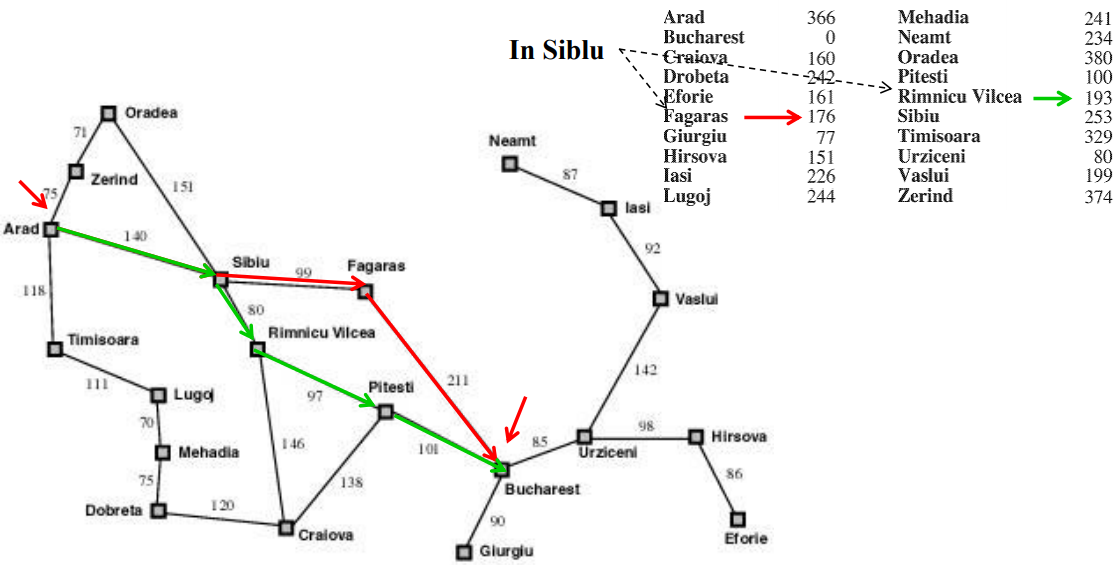
\includegraphics[width=0.8\textwidth]{immagini/greedy_bestFirst.png}
\end{figure}

Da Arad a Bucarest Greedy best-first:\ Arad, Sibiu, Fagaras, Bucharest (450); ma non è l'\textbf{ottimo}:\ Arad, Sibiu, Rimnicu, Pitesti, Bucarest (418).

\subsection{Algoritmo A:\ definizione}
Si può dire qualcosa di f per avere garanzie di completezza e ottimalità?\

\noindent \textit{Definizione}:\ un algoritmo A è un algoritmo \textbf{Best First} con una funzione di valutazione dello stato del tipo

\[f(n) = g(n) + h(n),\ \mathrm{con}\ h(n) \geq 0\ \mathrm{e}\ h(goal)=0\]

\begin{itemize}
	\item $g(n)$ è il costo del cammino percorso per raggiungere \textit{n};
	\item $h(n)$ una stima del costo per raggiungere da \textit{n} un nodo goal.
\end{itemize}
Vedremo come casi particolari dell'algoritmo A:\ se $h(n) = 0\ [f(n) = g(n)]$ si ha \textbf{Ricerca Uniforme} (\textbf{UC}), se $g(n) = 0\ [f(n) = h(n)]$ si ha \textbf{Greedy Best First}.

\begin{figure}[H]
	\centering
	\caption*{Esempio nel gioco dell'otto}
	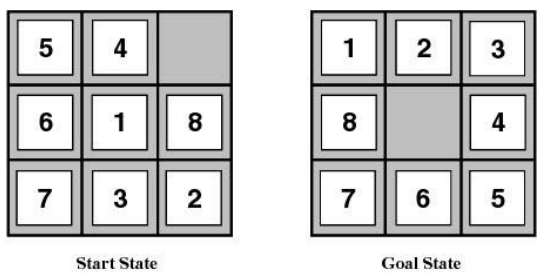
\includegraphics[width=0.6\textwidth]{immagini/otto_euristica.png}
\end{figure}

\noindent $f(n) = \#mosse fatte + \#caselle-fuori-posto$

\noindent $f(Start) = 0 + 7$ \qquad dopo $\leftarrow, \downarrow, \uparrow, \rightarrow\quad f = 4 + 7$

\noindent$f(goal state)=?+0$ stesso stato, \textit{g} è cambiata.

\subsubsection{L'algoritmo A è completo}

\begin{theorem}
	L'algoritmo A con la condizione
	\[ g(n) \geq d(n)\cdot \varepsilon \]
	dove $\varepsilon >0$ costo minimo arco e \textit{d} è la profondità, è completo.
\end{theorem}

\noindent\textbf{Nota}:\ la condizione ci garantisce che non si verifichino situazioni strane del tipo

\begin{figure}[H]
	\centering
	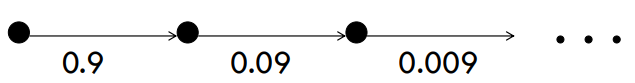
\includegraphics[width=0.5\textwidth]{immagini/AlgoritmoA_teorema.png}
\end{figure}

\noindent e che il costo lungo un cammino non cresca ``abbastanza''; se cresce abbastanza possiamo fermare quel path per costo alto di \textit{g}.

\begin{proof}[Dimostrazione di completezza]

	Sia $[n_0\ n_1\ n_2\ \dots\ n'\ \dots\ n_k = goal]$ un cammino soluzione.\
	Sia $n'$ un nodo della frontiera su un cammino soluzione:\ $n'$ prima o poi sarà espanso, infatti esistono solo un numero finito di nodi \textit{x} che possono essere aggiunti alla frontiera con $f(x) \leq f(n')$ (è la condizione sulla crescita di \textit{g} t.c.\ non esista una catena infinita di archi e nodi che possa aggiungere con costo sempre $\leq f(n')$).

	Quindi, se non si trova una soluzione prima, $n'$ verrà espanso e i suoi successori aggiunti alla frontiera, tra questi anche il suo successore sul cammino soluzione.\
	Il ragionamento si può ripetere fino a dimostrare che anche il nodo goal sarà selezionato per l'espansione.

\end{proof}

\subsection{Algoritmo A*}

\subsubsection{La stima ideale}
\begin{flushleft}
	Funzione di valutazione ideale (oracolo):

	\[f^*(n) = g^*(n) + h^*(n)\]

	$g^*(n)$ costo del cammino minimo da radice a n.

	$h^*(n)$ costo del cammino minimo da n a goal.

	$f^*(n)$ costo del cammino minimo da radice a goal, attraverso n.
\end{flushleft}

\noindent Normalmente:\ $g(n) \geq g^*(n)$ e $h(n)$ è una stima di $h^*(n)$.\
Si può andare in sottostima (e.g.\ linea d'aria) o sovrastima della distanza dalla soluzione.

\begin{definition}
	Si dice che un euristica è ammissibile se
	\[
		\forall n.\ h(n) \leq h^*(n)
	\]
	\textit{h} è una \textbf{sottostima}.\
	Per esempio l'euristica della distanza in linea d'aria.

\end{definition}

\begin{definition}
	Un \textbf{Algoritmo A*} è un algoritmo A in cui \textit{h} è una funzione euristica ammissibile.\
\end{definition}

\begin{theorem}
	Gli algoritmi A* sono \textbf{\textit{ottimali}}.
\end{theorem}

\begin{corollario}
	BF (con passi a costo costante) e UC sono ottimali \[h(n)=0\].\
\end{corollario}

\subsubsection{Itinerario con A*}
\begin{figure}[H]
	\centering
	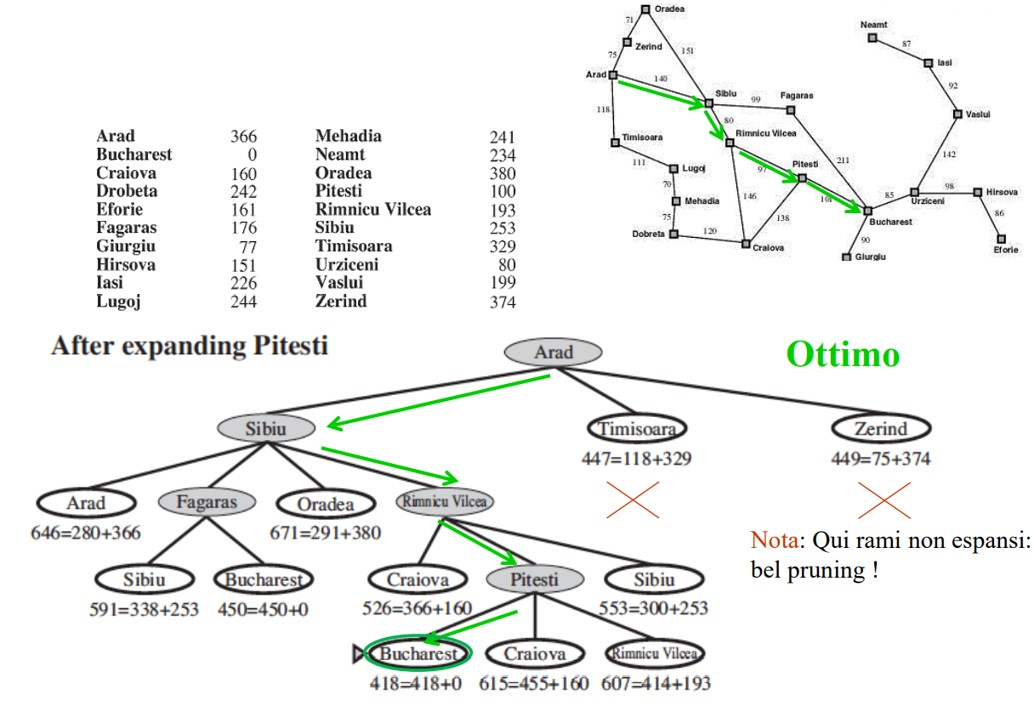
\includegraphics[width=\textwidth]{immagini/ItinerarioA.jpg}
\end{figure}

\subsubsection{Osservazioni su A*}

\begin{enumerate}
	\item Rispetto a greedy best-first, la componente \textit{g} fa sì che si abbandonino cammini che vanno troppo in profondità.
	\item \textit{h} sotto o sovra-stima?
	      \begin{itemize}
		      \item Una sottostima (\textit{h}) può farci compiere del lavoro inutile (tenendo anche candidati non buoni), però non ci fa perdere il cammino migliore (quando prendo nodo goal è il cammino migliore).
		      \item Una funzione che qualche volta sovrastima può farci perdere la soluzione ottimale (taglio per causa di sovrastima, invece era buona).
	      \end{itemize}
\end{enumerate}

\subsubsection{Ottimalità di A*}
Nel caso di ricerca a/su albero l'uso di un'euristica \textit{ammissibile} è sufficiente a garantire l'ottimalità di A*.\
Nel caso di ricerca su grafo serve una proprietà più forte, la \textbf{consistenza} (detta anche \textbf{monotonicità}), per evitare il rischio di scartare candidati ottimi (stato già incontrato) a causa dell'uso della lista esplorati che fa ``sparire'', o meglio, non considera candidati ottimali al momento dell'espansione.\
Cerchiamo quindi condizioni per garantire che il primo \textit{espanso} sia il migliore.

\subsection{Euristica consistente o monotòna}

\textit{Definizione}:\ euristica \textbf{consistente}
\begin{table}[H]
	\centering
	\begin{tabular}{l l}
		$[ h(goal) = 0 ]$                          &                                          \\
		$\forall n.\ h(n)\leq c(n, a, n') + h(n')$ & dove $n'$ è un successore di \textit{n}.
	\end{tabular}
\end{table}
\noindent Ne segue che $f(n) \leq f(n')$.\

\begin{figure}[H]
	\centering
	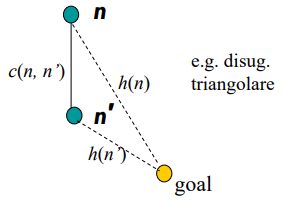
\includegraphics[width=0.4\textwidth]{immagini/eu_consistente.png}
\end{figure}

\noindent\textbf{Nota}:\ se \textit{h} è consistente la \textit{f} non decresce mai lungo i cammini, da cui il termine \textbf{monotòna}.

\subsubsection{Proprietà}
\textit{Teorema}:\ Un'euristica monotona è ammissibile.\

\noindent Esistono euristiche ammissibili che non sono monotone, ma sono rare*.\

Le euristiche monotone garantiscono che \textbf{la soluzione meno costosa venga trovata per prima} e quindi sono ottimali anche nel caso di ricerca su grafo.\ Non si devono recuperare tra gli antenati nodi con costo minore:\ lista degli esplorati, stato già esplorato è sul cammino ottimo $\rightarrow$ posso evitare di inserire il corrente ripetuto senza perdere l'\textit{ottimalità}.

\begin{flushleft}
	\textbf{if} \textit{figlio}.Stato non è in \textit{esplorati} e non è in \textit{frontiera} \textbf{then}

	\quad \textit{frontiera} = Inserisci(\textit{figlio}, \textit{frontiera})\newline

	Per la frontiera, volendo evitare stati ripetuti, resta ``\textit{if}'' finale di UC

	\textbf{if} \textit{figlio}.Stato è in \textit{frontiera} con \textit{Costo-cammino più alto} \textbf{then}

	\quad sostituisci quel nodo frontiera con \textit{figlio}
\end{flushleft}

\subsection{Ottimalità di A*}

Se $h(n)$ è consistente i valori di $f(n)$ lungo un cammino sono non decrescenti:
\begin{table}[H]
	\centering
	\begin{tabular}{l l}
		Se $h(n) \leq c(n, a, n') + h(n')$             & def. consistenza                  \\
		$g(n) + h(n) \leq g(n) + c(n, a, n') + h(n') $ & sommando $g(n)$                   \\
		ma siccome $g(n) + c(n, a, n') = g(n')$        &                                   \\
		$g(n) + h(n) \leq g(n') + h(n')$               &                                   \\
		$ \qquad \qquad f(n) \leq f(n')$               & $\rightarrow$ f \textbf{monotòna} \\
	\end{tabular}
\end{table}

\noindent Ogni volta che A* seleziona un nodo (\textit{n}) per l'\textit{espansione}, il cammino ottimo a tale nodo è stato trovato:\
se così non fosse, ci sarebbe un altro nodo $n'$ della frontiera sul cammino ottimo (che va a \textit{n} con un cammino ottimo ancora da trovare) con $f(n')$ minore (per la monotonia e \textit{n} successore di $n'$); ma ciò non è possibile perché tale nodo sarebbe già stato espanso (si espande prima un nodo con \textit{f} minore).\

Quando seleziona nodo goal è cammino ottimo ($h=0, f=C^*$).

\vspace{12pt}

\noindent Perché A* è vantaggioso?
\begin{itemize}
	\item A* espande tutti i nodi con $f(n)<C^*$ (\textit{C*} = costo ottimo)
	\item A* espande alcuni nodi con $f(n) = C^*$
	\item \textbf{A* non espande alcun nodo con} $f(n) > C^*$
\end{itemize}
Quindi alcuni nodi (e suoi sottoalberi) non verranno considerati per l'espansione (ma restiamo ottimali):\ \textbf{\textit{pruning}} (\textit{h} opportuna, più alta possibile tra le ammissibili, fa tagliare molto).
\begin{figure}[H]
	\centering
	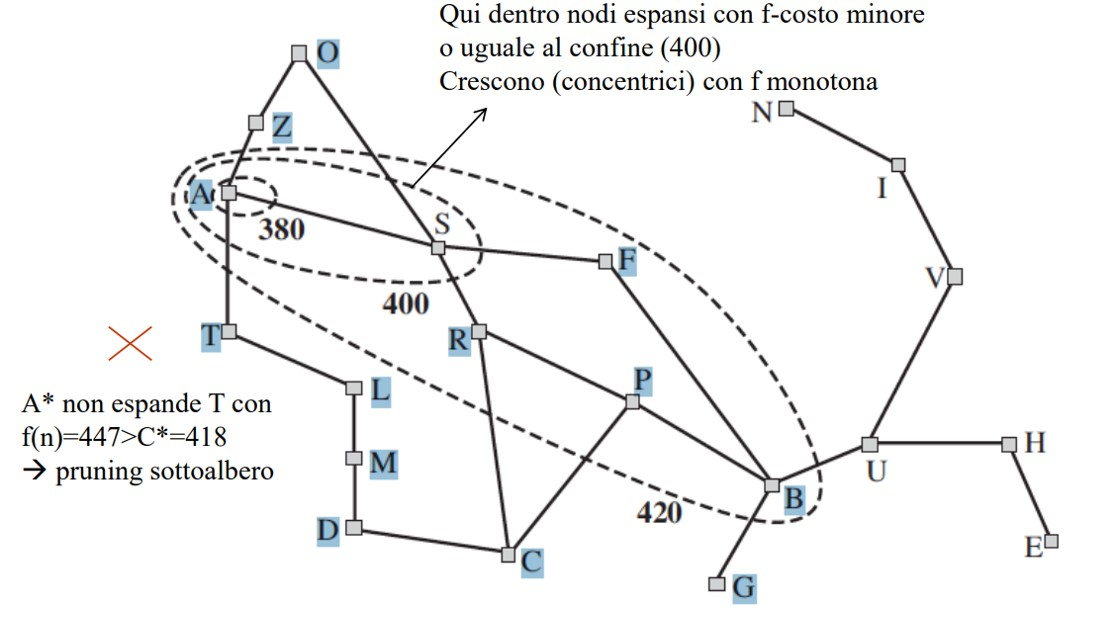
\includegraphics[width=0.8\textwidth]{immagini/Pruning.jpg}
\end{figure}
\noindent Più \textit{f} è aderente a stima ottimale, più taglio! Ovali più stretti.\ Cercheremo quindi una \textit{h} il più alta possibile tra le ammissibili.\
Se molto bassa molti (sino a tutti i) nodi restano minore di C* $\rightarrow$ espando tutti (a cerchi).\
Il pruning sotto-alberi è il punto focale:\ non li abbiamo già in memoria e evitiamo di generarli (decisivo per i problemi di AI a spazio stati esponenziali).

\subsubsection{Bilancio su A*}
\begin{itemize}
	\item A* è \textbf{completo}:\ discende dalla completezza di A (A* è un algoritmo A particolare).
	\item A* con euristica monotona è \textbf{ottimale}.
	\item A* è \textbf{ottimamente efficiente}:\ a parità di euristica nessun altro algoritmo espande meno nodi (senza rinunciare a ottimalità).
\end{itemize}
Problemi:\ ``Quale euristica?'' e ancora l'occupazione di memoria ($O(b^{d+1})$).

\subsection{Su \textit{f}:\ Due sotto-casi speciali}

\subsubsection{Casi particolari dell'algoritmo A}
\begin{itemize}
	\item Se $h(n) = 0\ [f(n) = g(n)]$ si ha Uniform Cost, ossia \textit{g} non basta.
	\item Se $g(n) = 0\ [f(n) = h(n)]$ si ha Greedy Best First, ossia \textit{h} non basta (già visto all'inizio).
\end{itemize}

\subsubsection{Dijkstra}
L'algoritmo A* è una generalizzazione dell'algoritmo di Dijkstra che riduce la dimensione del sottografo che deve essere esplorato, se è disponibile un limite inferiore sulla ``distanza'' dal bersaglio (h).

\newpage

\section{(Costruire) le euristiche di A*}

\subsubsection{Valutazione di funzioni euristiche}

A parità di ammissibilità, una euristica può essere più efficiente di un'altra nel trovare il cammino soluzione migliore (visitare meno nodi).\
Questo dipende da quanto \textit{informata} è l'euristica (dal \textbf{\textit{grado di informazione posseduto}}).
\begin{table}[H]
	\centering
	\begin{tabular}{l l}
		$h(n)=0$ & minimo di informazione (BF o UC)                     \\
		$h^*(n)$ & massimo di informazione (oracolo)                    \\
		\multicolumn{2}{c}{In generale, per le euristiche ammissibili:} \\
		\multicolumn{2}{c}{$0 \leq h(n) \leq h^*(n)$}                   \\
	\end{tabular}
\end{table}

\subsubsection{Più informata, più efficiente}

\begin{theorem}
	Se $h_1 \leq h_2$, i nodi espansi da A* con $h_2$ sono un sottoinsieme di quelli espansi da A* con $h_1$.
\end{theorem}

\noindent A* espande tutti i nodi con $f(n)= g(n)+h(n) <C^*$, e sono meno per \textit{h} maggiore (\textit{h} maggiore fa andare più nodi oltre C*).\
Se $h_1 \leq h_2$, A* con $h_2$
è almeno efficiente quanto A* con $h_1$.\
Un'euristica più informata (accurata) riduce lo spazio di ricerca (è più efficiente), ma è tipicamente più costosa da calcolare.

\subsubsection{Confronto di euristiche ammissibili}

Due euristiche ammissibili per il gioco dell'8
\begin{itemize}
	\item $h_1$:\ conta il numero di caselle fuori posto
	\item $h_2$:\ somma delle distanze Manhattan\footnote{$h((x,y)) = MD((x, y), (x_g , y_g)) = \mid x - x_g \mid + \mid y - y_g\mid$} (orizz./vert.) delle caselle fuori posto dalla posizione finale.
\end{itemize}
$h_2$ \textit{è più informata di} $h_1$, infatti $\forall n.\ h_1(n) \leq h_2 (n)$.

\noindent\textbf{\textit{Definizione}}:\ $h_2$ \textit{domina} $h_1$.

\begin{figure}[H]
	\centering
	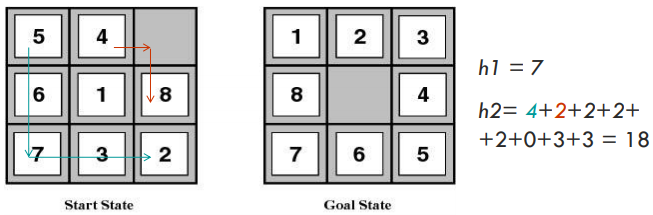
\includegraphics[width=0.8\textwidth]{immagini/otto_manhattan.png}
\end{figure}

\begin{figure}[H]
	\centering
	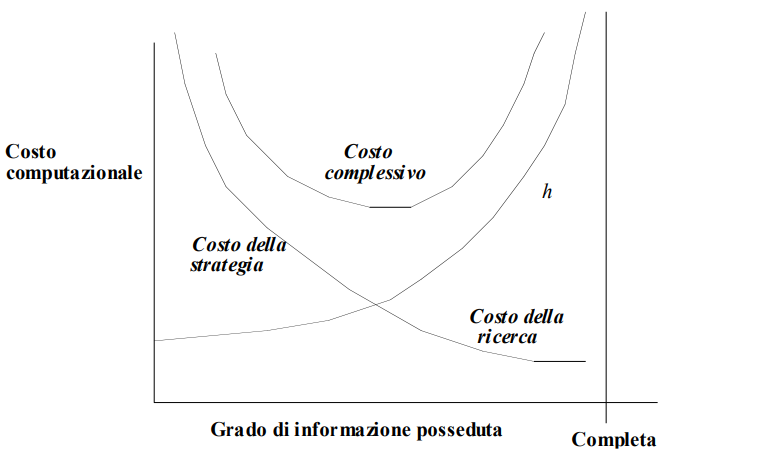
\includegraphics[width=\textwidth]{immagini/ricerca_euristica.png}
	\caption*{Costo ricerca vs costo euristica}
	\label{fig:my_label}
\end{figure}

\subsection{Misura del potere euristico}

Come valutare gli algoritmi di ricerca euristica\dots
\begin{center}
	\textit{Fattore di diramazione effettivo \textbf{b*}}

	\textit{N}:\ numero di nodi generati

	\textit{d}:\ profondità della soluzione
\end{center}
\textbf{\textit{b*}} è il fattore di diramazione di un albero uniforme con N+1 nodi; soluzione dell'equazione
\[
	N + 1=b^*+(b^*)^2+ \dots + (b^*)^d
\]
Sperimentalmente una buona euristica ha un \textit{b*} abbastanza vicino a 1 ($<$ 1.5).

\begin{table}[H]
	\centering
	\begin{tabular}{|c|c|c|c|}
		\hline
		d     & ID (appr. it. non inf)  & A*($h_1$)           & A*($h_2$)           \\\hline\hline
		2     & 10 (\textbf{2,43})      & 6 (\textbf{1,79})   & 6 (\textbf{1,79})   \\ \hline
		4     & 112 (\textbf{2,87})     & 13 (\textbf{1,48})  & 12 (\textbf{1,45})  \\ \hline
		6     & 680 (\textbf{2,73})     & 20 (\textbf{1,34})  & 18 (\textbf{1,30})  \\ \hline
		8     & 6384 (\textbf{2,80})    & 39 (\textbf{1,33})  & 25 (\textbf{1,24})  \\ \hline
		10    & 47127 (\textbf{2,79})   & 93 (\textbf{1,38})  & 39 (\textbf{1,22})  \\ \hline
		12    & 3644035 (\textbf{2,78}) & 227 (\textbf{1,42}) & 73 (\textbf{1,24})  \\\hline
		14    & -                       & 539 (\textbf{1,44}) & 113 (\textbf{1,23}) \\ \hline
		\dots & \dots                   & \dots               & \dots               \\ \hline
	\end{tabular}
	\captionsetup{singlelinecheck=off}
	\caption*{\begin{center}
			Esempio:\ dal gioco dell'otto
		\end{center}
		Sono riportati:\ nodi generati e fattore di diramazione effettivo (\textbf{\textit{b*}}).\ I dati sono mediati, per ogni d, su 100 istanze del problema.}
\end{table}

\subsubsection{Capacità di esplorazione}
Influenza di \textbf{\textit{b*}}:

\noindent \qquad Con $b=2$
\begin{table}[H]
	\centering
	\begin{tabular}{l l l}
		d=6  &              & N=100    \\
		d=12 & $\leftarrow$ & N=10.000 \\
	\end{tabular}
\end{table}

\noindent \qquad con $b=1.5$
\begin{table}[H]
	\centering
	\begin{tabular}{l l l}
		d=12 &              & N=100    \\
		d=24 & $\leftarrow$ & N=10.000 \\
	\end{tabular}
\end{table}

\noindent Migliorando di poco l'euristica si riesce, a parità di nodi espansi, a raggiungere una profondità doppia!

\noindent Quindi\dots
\begin{enumerate}
	\item Tutti i problemi dell'IA (o quasi) sono di complessità esponenziale\dots\ (nel generare nodi, i.e. configurazioni possibili) ma c'è esponenziale e esponenziale!
	\item L'euristica può migliorare di molto la capacità di esplorazione dello spazio degli stati rispetto alla ricerca cieca
	\item Migliorando anche di poco l'euristica si riesce ad esplorare uno spazio molto più grande (più in profondità).
\end{enumerate}

\subsection{Come si inventa un'euristica?}

Alcune strategie per ottenere euristiche ammissibili:
\begin{itemize}
	\item Rilassamento del problema
	\item Massimizzazione di euristiche
	\item Database di pattern disgiunti
	\item Combinazione lineare
	\item Apprendere dall'esperienza
\end{itemize}
\subsubsection{Rilassamento del problema}
Nel gioco dell'8 mossa da A a B possibile se
\begin{enumerate}
	\item B adiacente a A
	\item B libera
\end{enumerate}
$h_1$ e $h_2$ sono calcoli della distanza esatta della soluzione in versioni semplificate del puzzle:
\begin{itemize}
	\item $h_1$ (nessuna restrizione, ne 1 ne 2):\ sono sempre ammessi scambi a piacimento tra caselle (si muove ovunque) $\rightarrow$ \#caselle fuori posto.
	\item $h_2$ (solo restrizione 1):\ sono ammessi spostamenti anche su caselle occupate, purché adiacenti $\rightarrow$ somma delle distanze Manhattan.
\end{itemize}

\subsubsection{Massimizzazione di euristiche}

Se si hanno una serie di euristiche ammissibili
$h_1,\ h_2,\ \dots,\ h_k$ \textbf{senza che nessuna ``domini'' un'altra} allora conviene prendere il massimo dei loro valori:
\begin{center}
	$h(n)=\max\left\{(h_1(n),\ h_2(n),\ \dots,\ h_k(n))\right\}$
\end{center}
Se le $h_i$ sono ammissibili anche la \textit{h} lo è.\
La \textit{h} domina tutte le altre.

\subsubsection{Euristiche da sottoproblemi}

\begin{figure}[H]
	\centering
	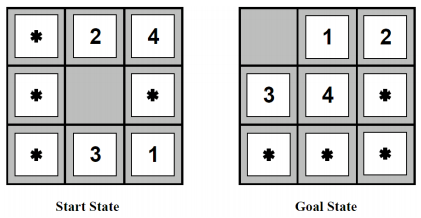
\includegraphics[width=0.6\textwidth]{immagini/sottoproblemi.png}
\end{figure}

Costo della soluzione ottima al sottoproblema (di sistemare 1,2,3,4) è una sottostima del costo per il problema nel suo complesso (rilevatesi più accurata della Manhattan).\

\textit{Database di pattern}:\ memorizzare ogni istanza del sotto\-problema con re\-lativo costo della soluzione.\
Usare questo database per calcolare \textit{h}\textsubscript{DB} (estraendo dal DB la configurazione corrispondente allo stato completo corrente).\
Potremmo poi fare la stessa cosa per altri sottoproblemi:\ 5-6-7-8, 2-4-6-8, \dots\ ottenendo altre euristiche ammissibili.\
Poi prendere il valore massimo:\ ancora una euristica ammissibile.

Ma potremmo sommarle e ottenere un'euristica ancora più accurata?

In generale no perchè le soluzioni ai sottoproblemi interferiscono (condividono alcune mosse, se sposto 1-2-3-4, spostero anche 4-5-6-7) e la somma delle euristiche in generale non è ammissibile (potremmo sovrastimare avendo avuto aiuti mutui).\
Si deve eliminare il costo delle mosse che contribuiscono all'altro sottoproblema.

Database di \textbf{pattern \textit{disgiunti}} consentono di sommare i costi (euristiche additive) [e.g. solo costo mosse su 1-2-3-4].\
Sono molto efficaci:\ gioco del 15 in pochi ms.\
Difficile scomporre per cubo Rubik.

\subsubsection{Apprendere dall'esperienza}

Far girare il programma, raccogliere dati:\ coppie $\langle \mathrm{stato},\ \mathrm{h^*} \rangle$.\
Usare i dati per apprendere a predire la \textit{h} con algoritmi di apprendimento induttivo (da istanze note stimiamo \textit{h in generale}).

Gli algoritmi di apprendimento si concentrano su caratteristiche salienti dello stato (\textit{feature}, \textit{x\textsubscript{i}}) [e.g.\ apprendiamo che da numero tasselli fuori posto 5 $\rightarrow$ costo $\sim$ 14, etc].

\subsubsection{Combinazione di euristiche}

Quando diverse caratteristiche influenzano la bontà di uno stato, si può usare una combinazione lineare
\[
	h(n)= c_1 x_1 (n) + c_2 x_2 (n) + \dots + c_k x_k (n)
\]
Gioco dell'8:
\[
	h(n)= c_1\ \#\mathrm{fuori\textrm{-}posto} + c_2\ \#\mathrm{coppie\textrm{-}scambiate}
\]
Scacchi:
\[
	h(n)= c_1\ \mathrm{vant\textrm{-}pezzi} + c_2\ \mathrm{pezzi\textrm{-}attacc.} + c_3\ \mathrm{regina} + \dots
\]
Il peso dei coefficienti può essere aggiustato con l'esperienza, anche qui apprendendo automaticamente da esempi di gioco.\
$h(goal) =0$ (e.g.\ gioco dell'8), ma ammissibilità e consistenza non automatiche.

\section{Algoritmi evoluti basati su A*}

\subsubsection{Beam search}

Nel Best First viene tenuta tutta la frontiera; se l'occupazione di memoria è eccessiva si può ricorrere ad una variante:\ la \textit{Beam search}.\
La \textbf{\textit{Beam Search}} tiene ad ogni passo solo \textit{i k nodi più promettenti}, dove \textit{k} è detto \textit{l'ampiezza del raggio} (\textit{beam}).

La \textit{Beam Search} non è completa.

\subsubsection{IDA*}
IDA* combina A* con ID:\ ad ogni iterazione si ricerca \textbf{in profondità} con un limite (cut-off) dato dal valore della \textbf{funzione \textit{f}} (e non dalla
profondità); il limite \textit{f-limit} viene aumentato ad ogni iterazione, fino a trovare la soluzione.\
Punto critico:\ di quanto viene aumentato \textit{f-limit}.

Cruciale la scelta dell'incremento per garantire l'ottimalità.\
Nel caso di costo delle azioni fisso è chiaro:\ il limite viene incrementato del costo delle azioni.\
Nel caso che i costi delle azioni siano variabili?\ Costo minimo oppure si potrebbe ad ogni passo fissare il limite successivo al valore minimo delle \textit{f} scartate (in quanto superavano il limite) all'iterazione precedente.

\noindent IDA* \textbf{completo} e \textbf{ottimale}
\begin{itemize}
	\item Se le azioni hanno costo costante \textit{k} (caso tipico 1) e \textit{f-limit} viene incrementato di \textit{k}.
	\item Se le azioni hanno costo variabile e l'incremento di \textit{f-limit} è $\leq \varepsilon$ (minimo costo degli archi)
	\item Se il nuovo \textit{f-limit} = min.\ valore \textit{f dei nodi generati ed esclusi all'iterazione precedente}.
\end{itemize}
Occupazione di memoria:\ $O(bd)$ [dall'algoritmo DF].

